\section{Strategy}\label{sec:strategy}

The proof has two limiting operations and then three ways of reading the same limiting correlations.
First we remove the lattice spacing while keeping the physical box fixed.
Then we enlarge the box, allowing a subsequence of volumes.
The later arguments recover relativistic fields, compare products at nearby points, and distinguish a two-point function from the specified free-field profiles.
None of them may replace the correlations obtained in the first two steps.

\paragraph{From small spacings to a fixed box.}
Refining the lattice adds new fluctuations at shorter distances.
We integrate these fluctuations a few scales at a time.
The resulting probability law is the effective law at the larger spacing; its coupling must be compared at one fixed reference spacing.
We adjust the bare coupling so that this reference coupling is always the same.
The observables must be adjusted along with the probability law; otherwise their correlations need not remain finite.
Proposition~\ref{prop:uv} produces one family of observables with these adjustments and proves their limits at each fixed volume.
Its estimates are local, so they can later control regions inside arbitrarily large boxes.

\paragraph{From boxes to phases.}
Local bounds independent of box size allow a subsequence on which the correlations converge.
This is the compactness step in Proposition~\ref{prop:limit}.
The result can still be an average of different states.
Reflection positivity turns its positive-time correlations into inner products, and averages at widely separated times distinguish its components.
After continuous rotations have been established, these averages commute and can be represented as functions on a compact space of phases.
Their expectation is integration against a probability measure, giving the mixture formula~\eqref{eq:mixture}.
The phase construction is therefore an additional argument after compactness.

\paragraph{Three conclusions from one hierarchy.}
Proposition~\ref{prop:reconstruction} selects a phase with a unique vacuum and continues its time variables to obtain relativistic fields.
Proposition~\ref{prop:ope} replaces a product at nearby points by a finite sum of fields at one point, with a controlled error inside any correlation with distant fields.
Its coefficients are chosen once, so the expansion also holds in every phase.
Proposition~\ref{prop:trace} studies the centred trace of the stress tensor: a logarithmic correction to its two-point singularity rules out the finite Wick profiles.
The dependence of these five results is summarised by
\begin{center}
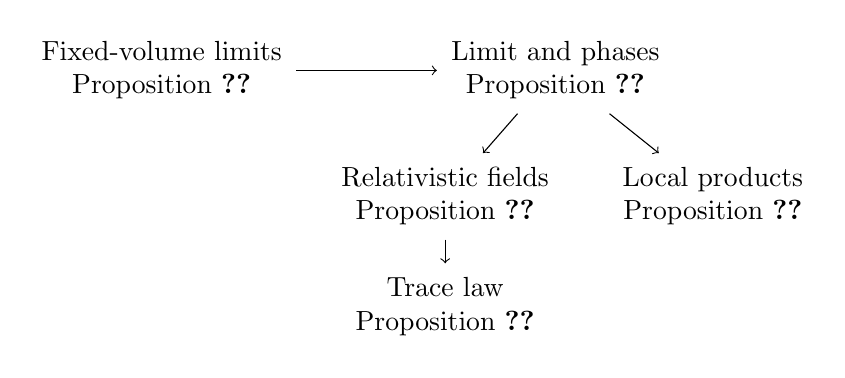
\begin{tikzpicture}[every node/.style={align=center,inner sep=5pt}]
\node (uv) at (0,0) {Fixed-volume limits\\Proposition~\ref{prop:uv}};
\node (limit) at (5,0) {Limit and phases\\Proposition~\ref{prop:limit}};
\node (reconstruction) at (3.6,-1.6) {Relativistic fields\\Proposition~\ref{prop:reconstruction}};
\node (ope) at (7,-1.6) {Local products\\Proposition~\ref{prop:ope}};
\node (trace) at (3.6,-3) {Trace law\\Proposition~\ref{prop:trace}};
\draw[->] (uv) -- (limit);
\draw[->] (limit) -- (reconstruction);
\draw[->] (limit) -- (ope);
\draw[->] (reconstruction) -- (trace);
\end{tikzpicture}
\end{center}
Here the last three results all use estimates for the same lattice family and the same continuum hierarchy supplied by the first two.
The arrows show the order of construction, not a claim that compactness alone gives their analytic inputs.

For each gauge group, we make one joint choice of the family in Proposition~\ref{prop:uv}.
For each prescribed increasing volume sequence, we then make one joint choice of a refinement and hierarchy for Propositions~\ref{prop:limit}--\ref{prop:trace}.
Their conclusions are not asserted for an arbitrary regular family or an arbitrary smooth table of correlations.
With these common choices, the deduction of Theorem~\ref{thm:main} is just the assembly of the five conclusions; it appears at the end of the next section.
